
\section{Experiments}\label{PARALLELXFASTTRIERESULTS}

For the experiments, we have again put in place a simple experimental protocol. We tested the three canonical operations: insertion, search and predecessor query, the ones that interest us the most, we can expect an equivalent time for successor or deletion requests. We compared the performance obtained for three different data structures, X-fast tries\index{X-fast trie}, B-trees and LSM\index{LSM}; each under special conditions.

For the insertions, the B-trees\index{B-tree} have no concurrent\index{Concurrent} version known as being really effective, we therefore reused the data structure developed in the chapter relating to X-fast tries$^{[\ref{BTREE}]}$ and this in a sequential\index{Sequential} context, i.e. with only one warp in only one block.

For LSM\index{LSM}, the situation is different, first, it is difficult to provide true parallelism to this data structure given its inherent sequentiality\index{Sequential} and, second, for technical reasons, we have not been able to launch more than 16 warps related to too much shared memory use for the sort primitive used.

Finally, for the X-fast tries, the problem was quite different, crashes appeared in some rare case. Of course, we investigated the reasons for these problems, but the bugs did not seem obvious to us. Nonetheless, we have been able to carry out a sufficient number of experiments and we may hope that the results would be representative of those actually obtained.

On the other hand, for queries, there is no reason to deprive ourselves of the parallelism offered by graphics cards\index{Graphics cards}, so we decided to use 16 warps and 32 blocks, which should be enough to saturate the streaming processors and therefore get the maximum theoretical performance. All tests were performed with pre-allocated memory and the hash tables\index{Hash table} had a capacity equal to twice the expected number of elements, thus a load factor of 50\%. We collected the results on 20 runs and 5 iterations.

\section{Results}

As usual, we will present each of the experiments that were conducted associated with its relative conclusions. The size of the points represents the standard deviation obtained in the results and their position the mean value.

We'll start with the insertions and we can observe several phenomena:

\begin{figure}[!htb]
    \centering
    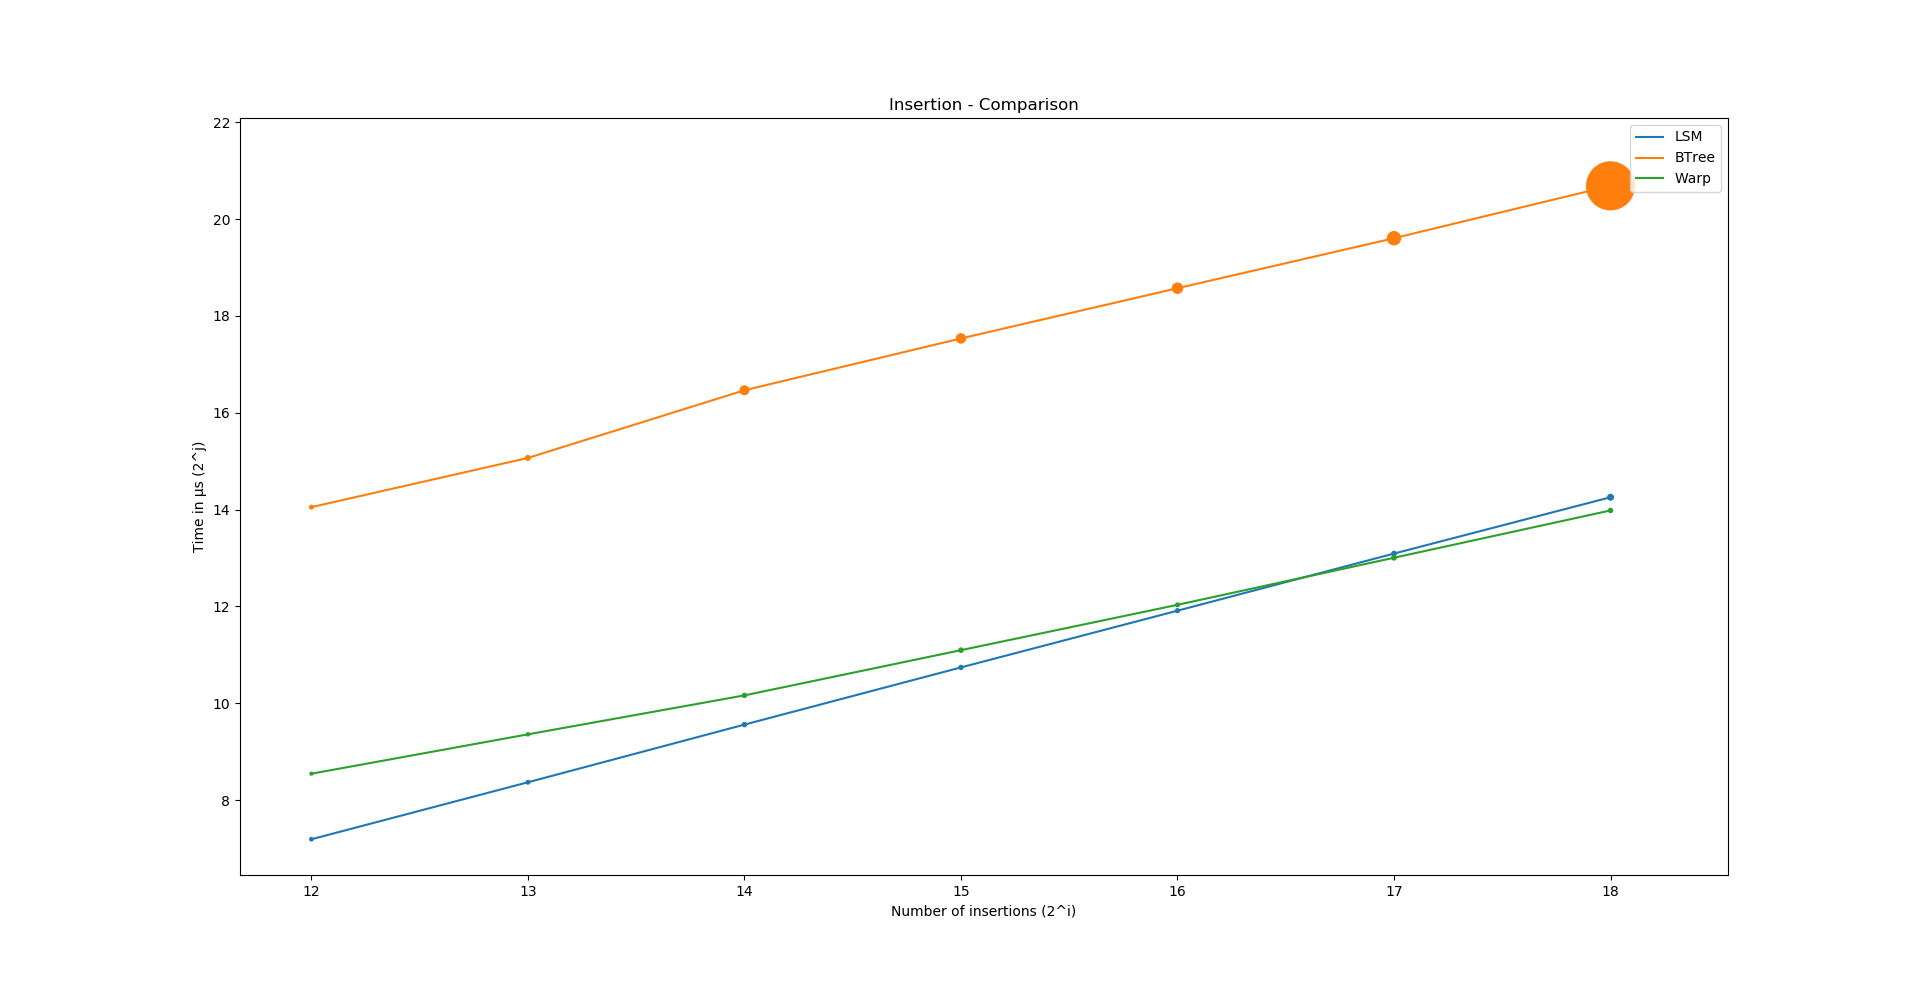
\includegraphics[width=\linewidth]{Chapters/ParallelXFastTries/Insertions.png} 
    \caption{32-bit key insertion}
\end{figure}

\begin{itemize}
    \item The standard deviation is a bit lower for X-fast tries\index{X-fast trie}. Indeed, it seems relatively clear that their variance is only dependent on the queries performed on the internal hash tables\index{Hash table}. But the load factor is relatively low, only 50\%, so it seems normal to have a narrow variance. On the contrary, we had already observed that the B-trees\index{B-tree} had a stronger tendency to have high variances related to the rebalancing necessary to maintain the structure in the tree. Finally, the LSM\index{LSM} have an associated variance relatively small in comparison to that of the B-trees\index{B-tree}, this is related to the cascading merge which must be carried out each time one passes to the next power of 2.
    \item The gain in concurrency that we have obtained by exploiting more warps for X-fast tries\index{X-fast trie} is very interesting. For both LSM\index{LSM} and X-fast tries\index{X-fast trie}, insertions are almost 100 times faster than for sequential B-trees\index{B-tree}.
    \item The LSM\index{LSM} offers lower starting constants but the coefficients of the larger orders seem larger. This does not seem so irrelevant since the merge operation is not totally without cost (the cost to sort the original buffer remains marginal~\cite{ashkiani2017parallel}). The LSM primitives are incredibly fast but the cascading mecanism remains significant on the performances.
    \item In this context, insertions in X-fast tries\index{X-fast trie} seem to be a good alternative to LSM\index{LSM}, following the batch size used of 512; and with greater flexibility, element-wise and not like in a bulk synchronous model. Note that the batch size presented in the original article was quite different, by a factor of more than 32 and that our implementation is not as optimal as their one.
\end{itemize}

We will continue with the two search operations:

We will start with thread-based queries:

\begin{figure}[!htb]
    \centering
    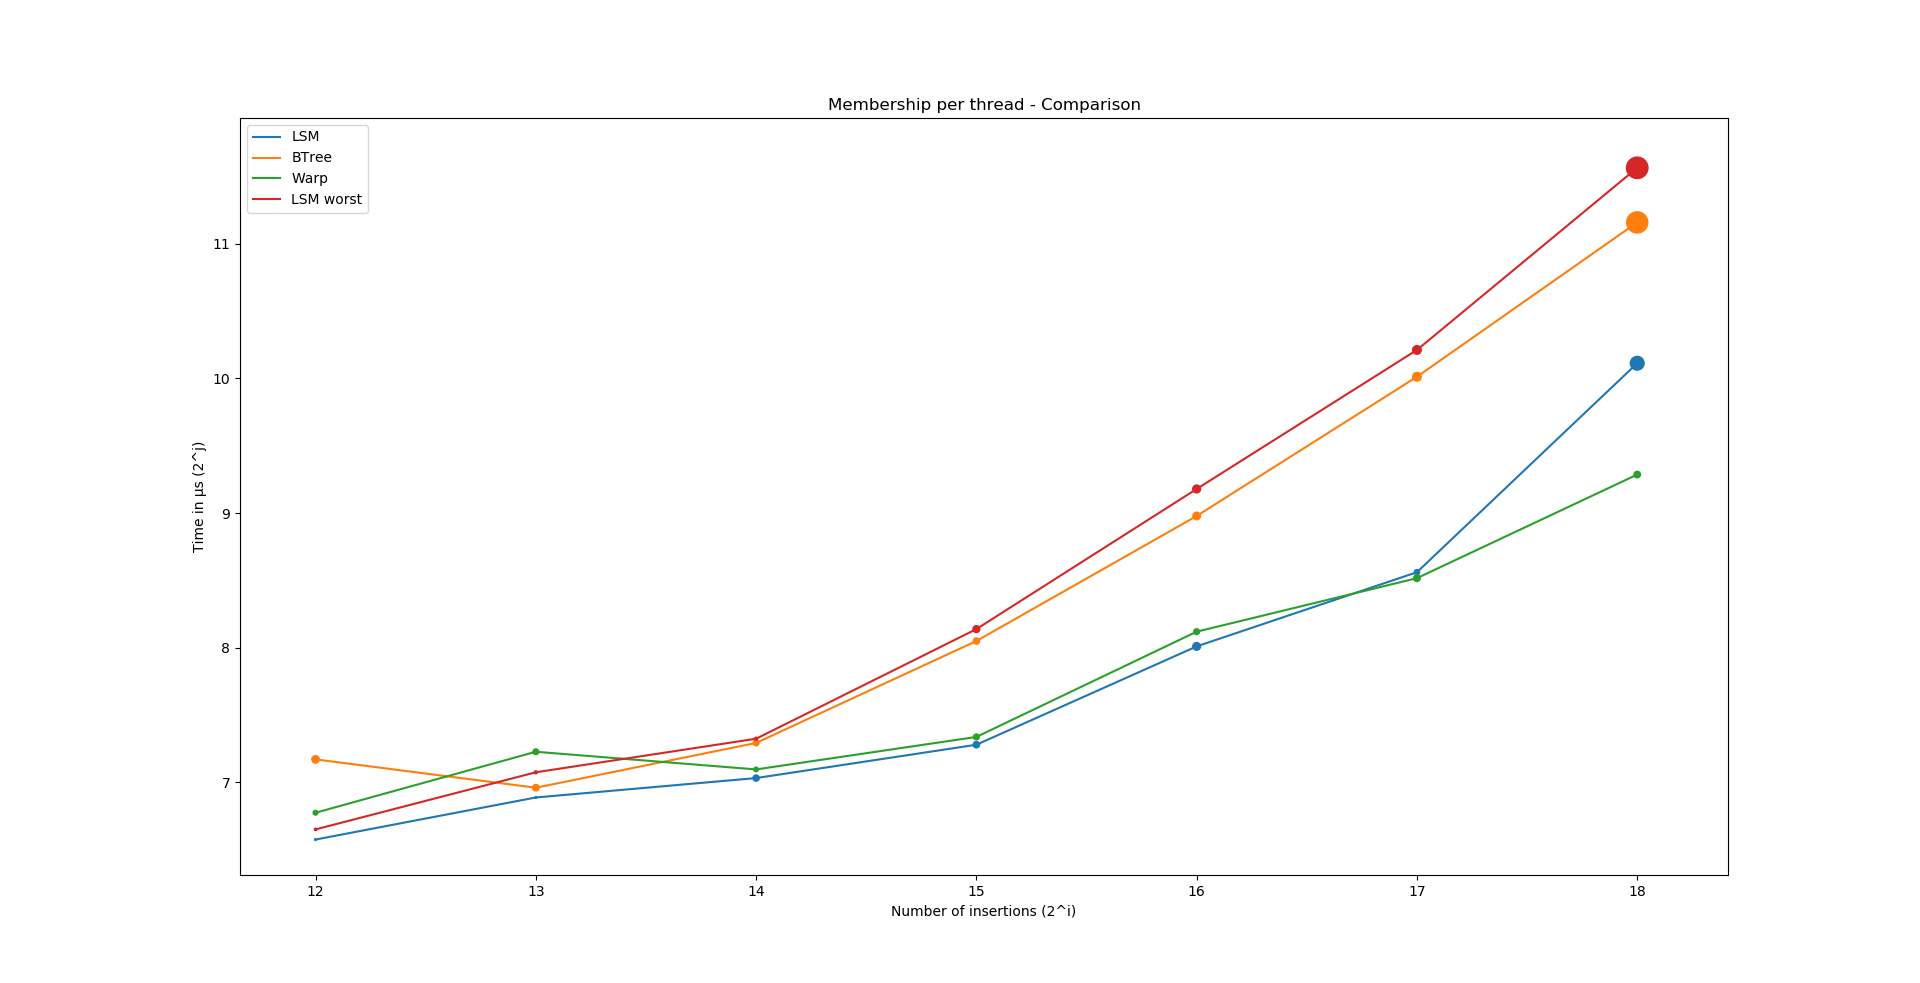
\includegraphics[width=0.85\linewidth]{Chapters/ParallelXFastTries/Membership_thread.png} 
    \caption{Thread-based searches}
\end{figure}

The results are somewhat astonishing:
\begin{itemize}
    \item Very logically, accessing X-fast tries\index{X-fast trie} elements is faster than for B-trees\index{B-tree}, since it consists of a simple search in a hash table\index{Hash table}, instead of running through an entire tree.
    \item But the difference between X-fast tries\index{X-fast trie} and LSM\index{LSM} is very surprising, they are really close. The main argument is related to the fact that the locality of the data is much stronger in the LSM\index{LSM}. The first pivots used during the dichotomous search, have strong chances to be kept in memory since they will be very often requested. We are also in the ideal situation for LSM where only one dichotomous search must be performed, since we have inserted a power of 2 elements ($b2^{k}$).
    \item When requests are made in the worst case for LSM, which corresponds to a number of insertions which is a power of 2 minus 1 ($b2^{k} - b$), the performances become comparable to that of a B-tree due to the potential $O(\log N)$ queries made. On average, the LSM remains better than the B-tree.
\end{itemize}

Now, the warp-based queries where the whole warp contributes to search one element:

\begin{figure}[!htb]
    \centering
    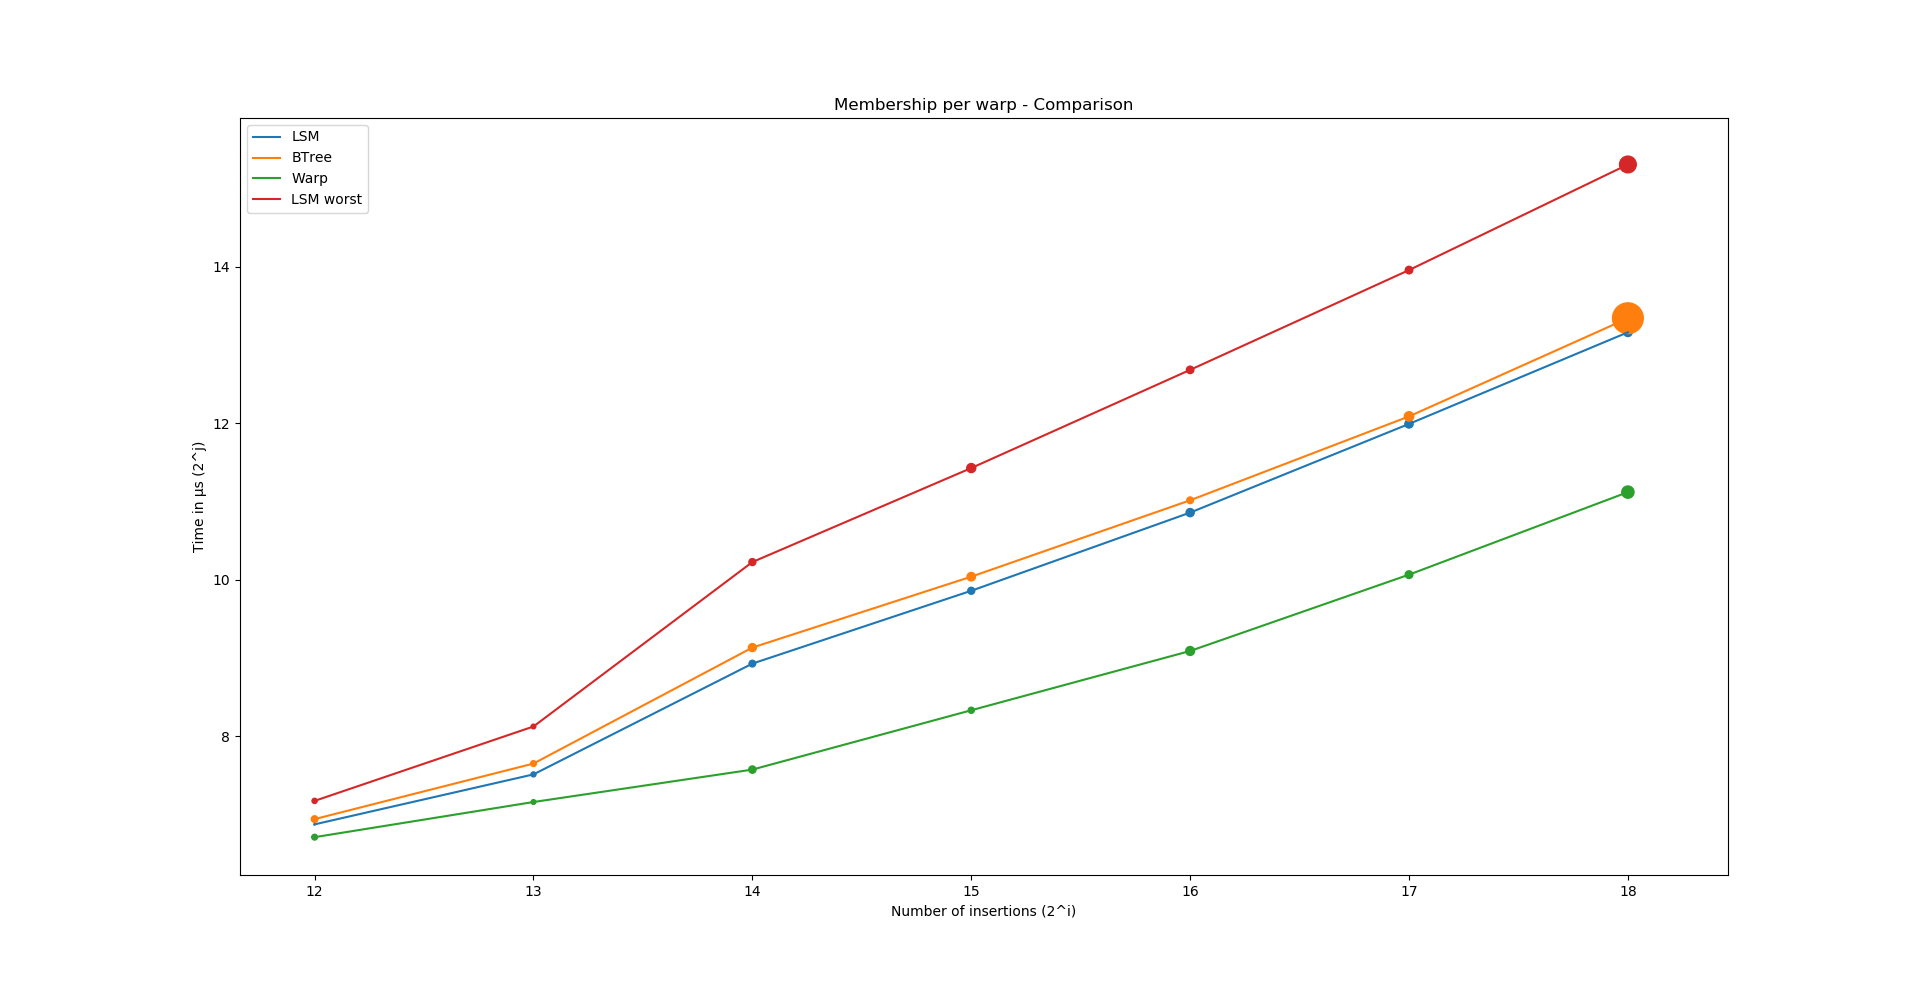
\includegraphics[width=0.85\linewidth]{Chapters/ParallelXFastTries/Membership_warp.png} 
    \caption{Warp-based searches}
\end{figure}

We observe similar phenomena:
\begin{itemize}
    \item The best case for LSM\index{LSM} is close to B-trees because dichotomous key searches no longer have to be performed. So all that remains is the cost of searching properly and loading the different blocks.
    \item X-fast tries\index{X-fast trie} retain their advantage thanks to the multiple probes performed at the same time in the leaf-level hash table\index{Hash table}.
\end{itemize}

\newpage

Finally, all we have left to observe are the predecessor's queries:

\begin{figure}[!htb]
    \centering
    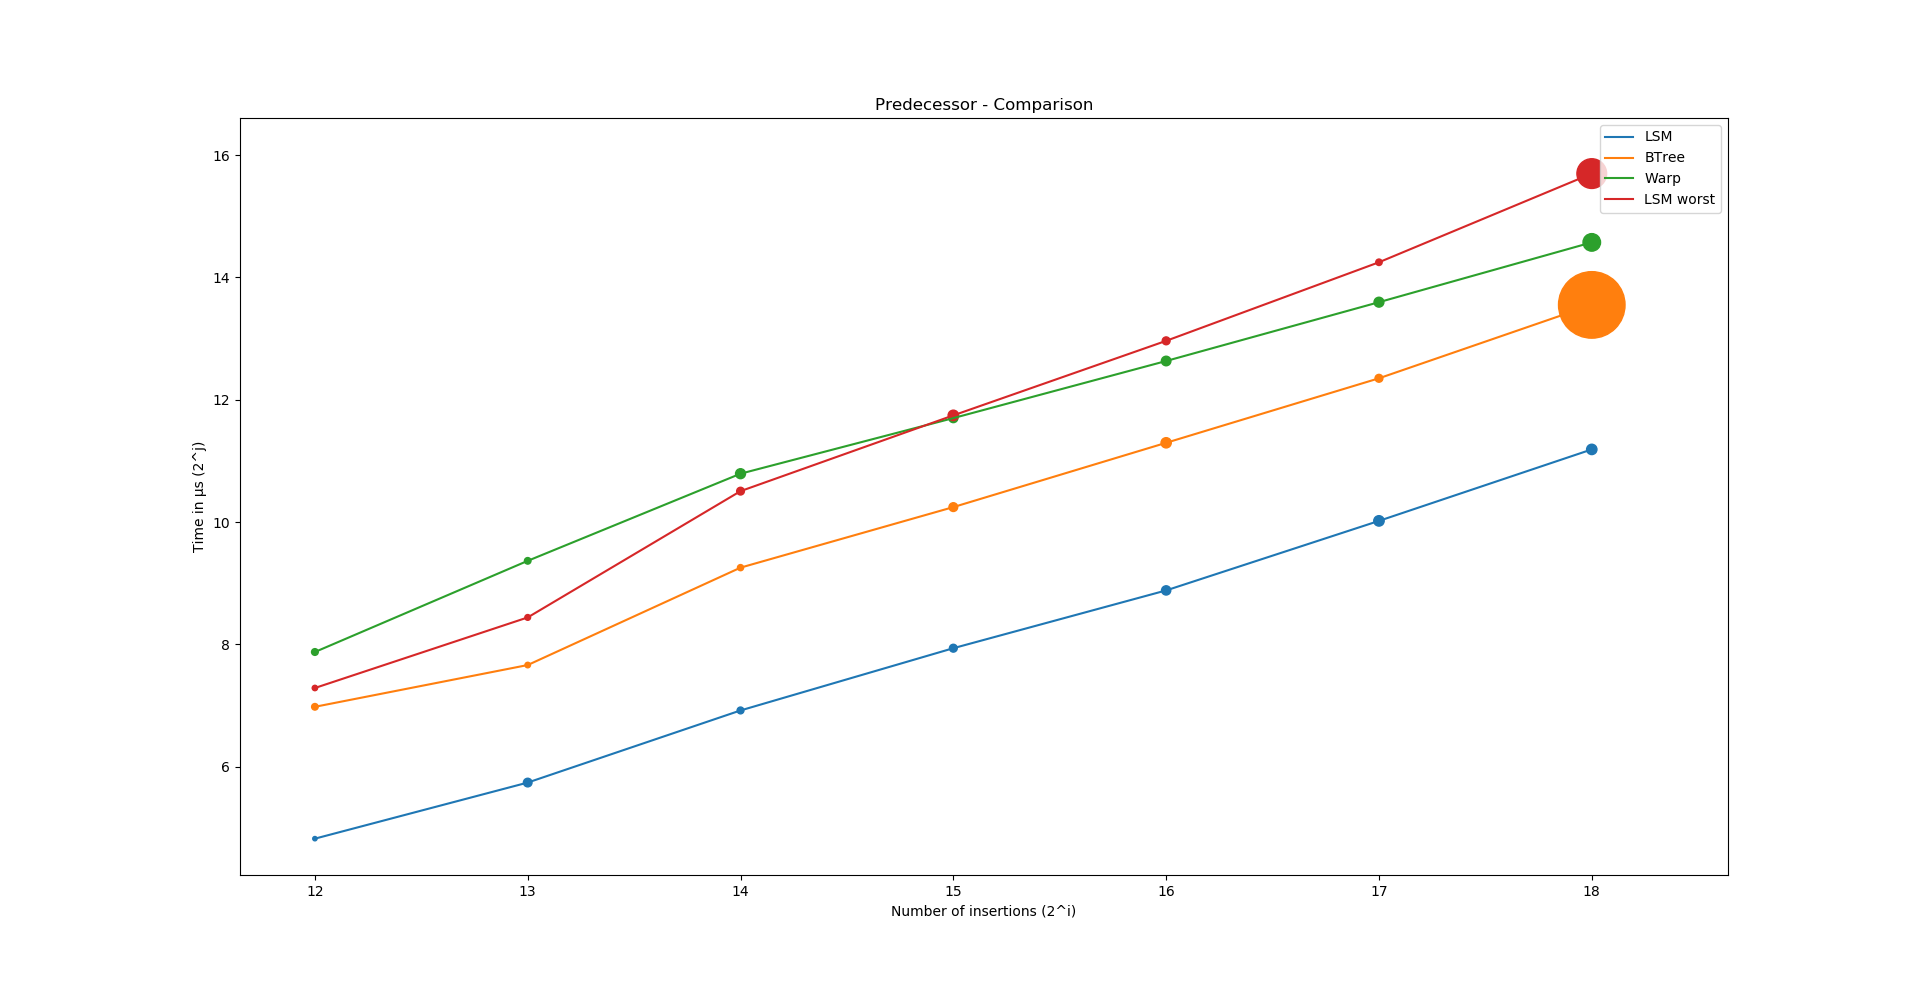
\includegraphics[width=\linewidth]{Chapters/ParallelXFastTries/Predecessor.png} 
    \caption{Warp-based predecessor queries}
\end{figure}

Some remarks can be made:
\begin{itemize}
    \item We notice the same phenomenon as in the sequential\index{Sequential} framework, X-fast tries\index{X-fast trie} are slower than B-trees\index{B-tree} because of their imposing number of memory requests.
    \item For the LSM\index{LSM}, the performance is roughly equivalent to the search operation, which is quite logical since both use lower bound algorithm.
    \item We precise that the predecessor search can be done by thread for LSM, whereas for X-fast tries, it can only be done by warp. So we simulated this operation by performing only one of the queries in the warp to make it comparable to other data structures.
    \item De facto, the time that would be taken to search for the predecessor per thread for LSM\index{LSM} would be even faster than pseudo warp-based, and a gain of a factor 8 would not seem excessive.
    \item Predecessor requests in X-fast tries are faster than those in a LSM in the worst case, but on average they are significantly slower.
\end{itemize}
